\chapter{Results and Discussion}

\section{Performance Evaluation of Different Image Transformation Techniques}

This section presents the findings of the experiment evaluating four image transformation techniques Spectrograms, GADF, GASF, and MTF for sleep stage classification using Vision Transformers. Figure \ref{fig:ts2img} provides a visual comparison of these methods applied to the same epoch. The classification performance was summarized in Table \ref{tab:transformation_methods_performences}. These findings offer insights into the most effective transformation method for PSG signal representation in Vision Transformer-based sleep stage classification.

\begin{figure}[H]
    \centering
    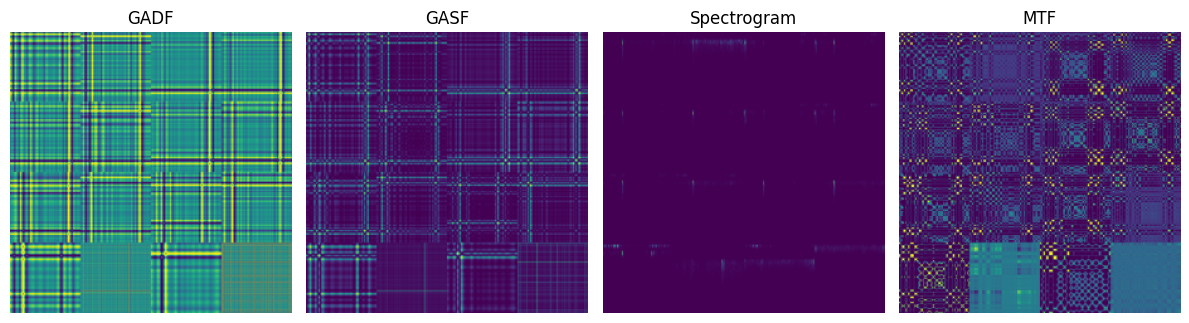
\includegraphics[width=1\linewidth]{Figures/ts2img.png}
    \caption{Visual representation of different image transformation techniques applied to sleep stage classification.}
    \label{fig:ts2img}
\end{figure} 

\begin{table}[H]
    \centering
    \resizebox{\textwidth}{!}{%
    \begin{tabular}{lcccc}
        \toprule
        \textbf{Transformation Method} & \textbf{Accuracy (\%)} & \textbf{F1-Score} & \textbf{Processing Time (s/epoch)} \\
        \midrule
        Spectrogram & 55.4 & 0.54  & 0.4 \\
        GADF        & 56.7 & 0.55  & 0.2 \\
        GASF        & 57.2 & 0.57  & 0.2 \\
        MTF         & 57.1 & 0.56  & 5 \\
        \bottomrule
    \end{tabular}%
    }
    \caption{Performance comparison of image transformation techniques for sleep stage classification.}
    \label{tab:transformation_methods_performences}
\end{table}

Among the tested methods, GASF achieved the highest accuracy (57.2\%) and F1-score (0.57), making it the most informative representation for the ViT-based classifier. MTF showed comparable accuracy (57.1\%) and F1-score (0.56), but its high processing time (5 seconds per epoch) makes it impractical for large-scale applications. GADF demonstrated moderate performance (Accuracy: 56.7\%, F1-score: 0.55) but was computationally efficient, requiring only 0.2 seconds per epoch. Spectrograms performed the worst (Accuracy: 55.4\%, F1-score: 0.54), indicating weak feature representation for ViT. \\

Overall, GASF is the most effective transformation, offering a balance between high classification performance and computational efficiency. While MTF provides similar accuracy, its high processing time limits its real-time usability. \\ 

To further assess each transformation technique, feature embeddings from the final layer of ViT-B/16 were extracted and visualized using t-Distributed Stochastic Neighbor Embedding (t-SNE). Figure \ref{fig:tsne_img} illustrates the t-SNE plots for all four methods. The t-SNE visualizations did not reveal clearly separable clusters, suggesting that t-SNE alone is insufficient for evaluating transformation distinctiveness. Therefore, clustering quality was assessed using Silhouette Score, Davies-Bouldin Index (DBI), and Calinski-Harabasz Index (CHI) (Table \ref{tab:transformation_methods_cluster_performences}). 

\begin{figure}[H]
    \centering
    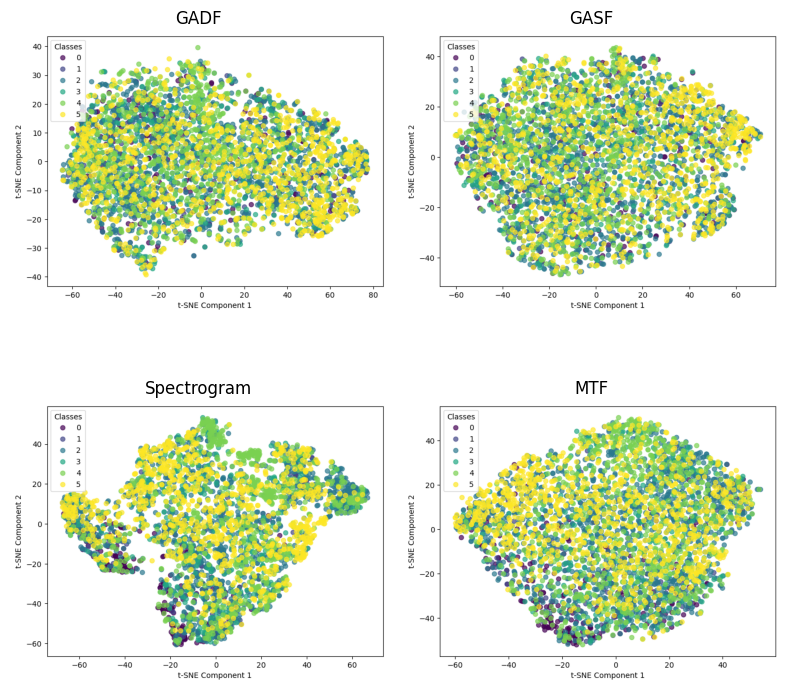
\includegraphics[width=0.8\linewidth]{Figures/tsne.png}
    \caption{t-SNE visualization of feature embeddings extracted from the ViT-B/16 for the GADF, GASF, Spectrogram, and MTF.}
    \label{fig:tsne_img}
\end{figure}

\begin{table}[H]
    \centering
    \resizebox{\textwidth}{!}{%
    \begin{tabular}{lcccc}
        \toprule
        \textbf{Transformation} & \textbf{Silhouette} & \textbf{Davies-Bouldin} & \textbf{Calinski-Harabasz}\\

        \textbf{Method} & \textbf{Score} & \textbf{Index} & \textbf{Index}\\
        \midrule
        Spectrogram & -0.05 & 45.44 & 20.41 \\
        GADF        & -0.07 & 10.51 & 49.70 \\
        GASF        & -0.08 & 10.45 & 53.79 \\
        MTF         & -0.07 & 23.88 & 19.76 \\
        \bottomrule
    \end{tabular}%
    }
    \caption{Clustering Performance for Different Image Transformations}
    \label{tab:transformation_methods_cluster_performences}
\end{table}

The Silhouette Score was negative for all methods, indicating poor clustering. Spectrograms had the highest score (-0.05), while GASF had the lowest (-0.08), suggesting weak cluster separability. The DBI showed that GASF (10.45) and GADF (10.51) achieved the best cluster separation, whereas Spectrograms (45.44) and MTF (23.88) exhibited substantial overlap. The CHI further confirmed GASF as the best method (53.79), followed by GADF (49.70), while Spectrograms (20.41) and MTF (19.76) demonstrated poor clustering performance. \\

Overall, GASF and GADF produced more structured and distinct clusters, making them better feature representations for sleep stage classification. Spectrograms and MTF exhibited weak clustering, aligning with the t-SNE findings. \\

Therefore, among the evaluated image transformation techniques, GASF emerged as the most effective, balancing high classification performance, computational efficiency, and structured feature representation. 


\section{Effect of Sampling Frequency and Resampling Method}

This section presents the findings on the impact of sampling frequency and resampling methods on sleep stage classification performance. Classification accuracy was evaluated across four sampling frequencies (512 Hz, 256 Hz, 128 Hz, and 64 Hz) and two resampling methods (FFT and DWT) to determine the most effective combination. Based on the results of Experiment 1, GADF was selected as the image transformation method. Figures \ref{fig:fft_img} and \ref{fig:dwt_img} visually represent the resampling methods at different frequencies applied to the same epoch. The results, summarized in Table \ref{tab:effect_of_frequency}, provide insights into how downsampling and resampling influence PSG signal representation for Vision Transformer-based classification.
\begin{figure}[H]
    \centering
    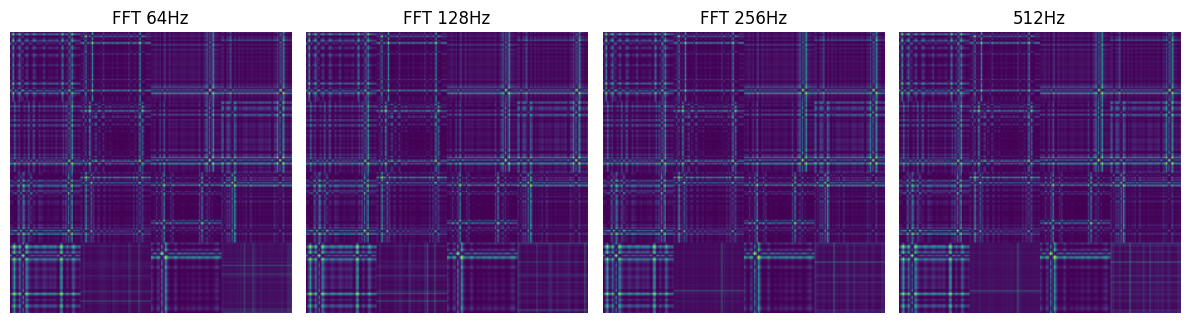
\includegraphics[width=1\linewidth]{Figures/fft.png}
    \caption{GASF representations at different sampling frequencies using Fast Fourier Transform.}
    \label{fig:fft_img}
\end{figure}

\begin{figure}[H]
    \centering
    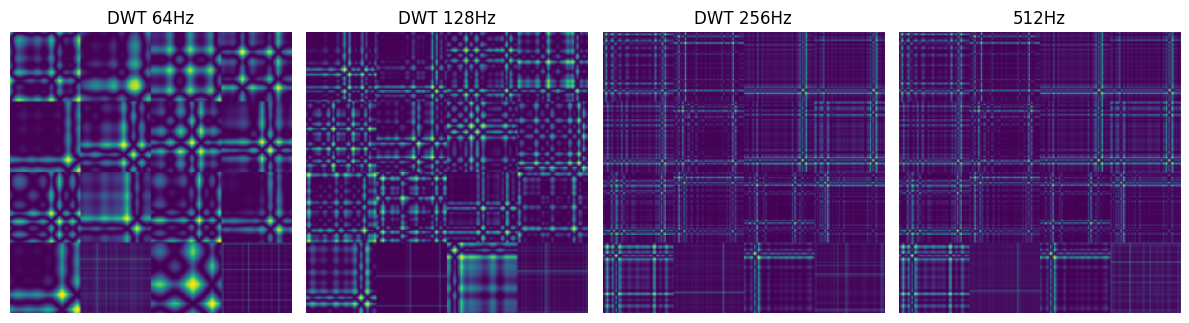
\includegraphics[width=1\linewidth]{Figures/dwt.png}
    \caption{GASF representations at different sampling frequencies using Discrete Wavelet Transform.}
    \label{fig:dwt_img}
\end{figure}

\begin{table}[H]
    \centering
    \resizebox{\textwidth}{!}{ % Resize to fit within page width
    \begin{tabular}{llcccc}
        \toprule
        \textbf{Sampling Frequency} & \textbf{Resampling Method} & \textbf{Accuracy (\%)} & \textbf{F1-Score} \\
        \midrule
        512 Hz & Original  & 57.2 & 0.57   \\
        256 Hz & FFT  & 58.0 & 0.57   \\
        256 Hz & DWT  & 58.5 & 0.58   \\
        128 Hz & FFT  & 56.3 & 0.55  \\
        128 Hz & DWT  & 60.1 & 0.60   \\
        64 Hz  & FFT  & 53.8 & 0.52   \\
        64 Hz  & DWT  & 56.4 & 0.56   \\
        \bottomrule
    \end{tabular}
    }
    \caption{Performance of sleep stage classification using different sampling frequencies and resampling methods.}
    \label{tab:effect_of_frequency}
\end{table}

The results indicate that down-sampling using DWT at 128 Hz achieved the highest performance, with an accuracy of 60.1\% and an F1-score of 0.60. This suggests that the combination of lower sampling frequency and the DWT resampling method enhances the model's ability to classify sleep stages accurately. Notably, DWT at 256 Hz also showed strong performance, with an accuracy of 58.5\% and an F1-score of 0.58, indicating that DWT offers better results compared to FFT for similar sampling frequencies. \\

In contrast, the FFT method at 128 Hz resulted in a lower accuracy of 56.3\% and F1-score of 0.55, suggesting that FFT may be less effective at lower sampling frequencies. Furthermore, the performance at 64 Hz was significantly lower, with an accuracy of 53.8\% and an F1-score of 0.52, particularly when using FFT. Even with the DWT method at 64 Hz, the performance was still lower (56.4\% accuracy, 0.56 F1-score), further highlighting the challenges of downsampling to very low frequencies. \\

Interestingly, the original 512 Hz data (without downsampling) achieved an accuracy of 57.2\% and an F1-score of 0.57, showing that while downsampling improves computational efficiency, it may come at the cost of classification accuracy—especially when using FFT. \\

Overall, the results suggest that DWT resampling provides the best trade-off between classification accuracy and computational efficiency, especially at 128 Hz and 256 Hz. FFT, on the other hand, tends to perform less effectively at lower sampling frequencies, especially when downsampling to 64 Hz.



\section{Effectiveness of Pre-Trained vs. From-Scratch ViTs}

This section presents the findings on the effectiveness of pre-trained versus from-scratch Vision Transformers (ViTs) for sleep stage classification. The experiments were conducted using both balanced and imbalanced datasets to evaluate the models’ generalization capabilities. Based on prior experiments, the Gramian Angular Summation Field (GASF) with Discrete Wavelet Transform (DWT) at 128 Hz was selected as the optimal image transformation method. \\ 

The from-scratch ViT model was developed after experimenting with various architectures and hyperparameter tuning to optimize sleep stage classification performance. Different configurations of embedding dimensions, attention heads, and transformer layers were explored to balance model complexity and generalization. The final architecture is summarized in Table \ref{tab:best_from_scratch}. \\

\begin{table}[H]
    \centering
    \begin{tabular}{l c}
        \toprule
        \textbf{Component} & \textbf{Details} \\
        \midrule
        Patch Size & 16 × 16 \\
        Embedding Dimension (D) & 256 \\
        Transformer Layers (L) & 6 \\
        Attention Heads & 8 \\
        MLP Hidden Dimension & 512 \\
        Dropout & 0.1 \\
        Classifier Head & Fully Connected (FC) + Softmax \\
        \bottomrule
    \end{tabular}
    \caption{ Summary of the Best Performing From-Scratch ViT Architecture}
    \label{tab:best_from_scratch}
\end{table}

Figure \ref{fig:fn_scrtach} illustrates the results, showing a clear performance advantage of the pre-trained ViT over the from-scratch model. The pre-trained ViT achieved a 78.1\% accuracy on the balanced dataset, outperforming the from-scratch ViT by 9.2\%. Similarly, for the imbalanced dataset, the pre-trained ViT obtained 68.5\% accuracy, which is 4.1\% higher than the from-scratch model.

\begin{figure}[H]
    \centering
    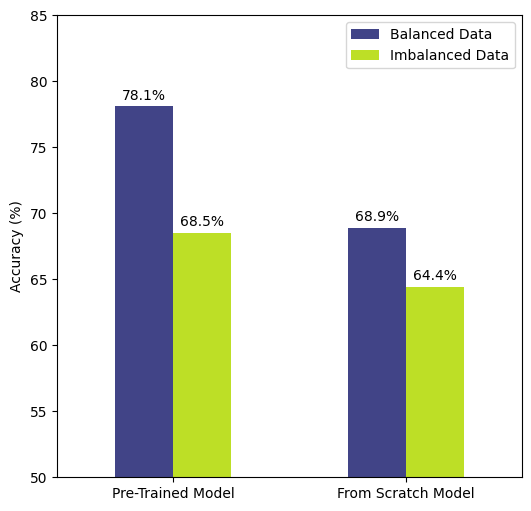
\includegraphics[width=0.6\linewidth]{Figures/fn_scratch.png}
    \caption{Comparison of Accuracy for Fine-Tuned and Model from Scratch on Balanced and Unbalanced Data}
    \label{fig:fn_scrtach}
\end{figure}

These results suggest that leveraging transfer learning with a pre-trained ViT significantly enhances classification accuracy, especially when data availability is limited or imbalanced. The superior performance of the pre-trained model highlights the benefits of prior feature extraction from large-scale datasets, enabling better generalization to sleep stage classification.

\section{Effectiveness of Different Pre-Trained Vision Transformers}

This section presents the findings on the effectiveness of different pre-trained Vision Transformer models for sleep stage classification. Building on previous experiments, a balanced image dataset was created using the DS9 dataset, and multiple pre-trained ViT models—ViT-B/16, ViT-B/32, DeiT-B, Swin-B, BEiT-B, and PVT-Small—were fine-tuned using a consistent preprocessing pipeline. The results, summarized in Table \ref{tab:pre_trained_models} and Figure \ref{fig:pretrained_models}, provide insights into the classification performance and computational efficiency of each model, helping identify the most suitable ViT architecture for sleep stage classification.

\begin{table}[H]
    \centering
    \resizebox{\textwidth}{!}{ % Resize to fit within page width
    \begin{tabular}{llcccc}
        \toprule
        \textbf{Model} & \textbf{Accuracy (\%)} & \textbf{F1-Score} & \textbf{Inference Time (ms/eppoch)} \\
        \midrule
        ViT-B/16 & 78.1  & 77.2 & 290   \\
        ViT-B/32 & 75.8  & 73.9 & 320   \\
        DeiT-B	 & 76.4  & 74.5 & 250   \\
        Swin-B	 & 77.9  & 76.1 & 280  \\
        BEiT-B	 & 77.2  & 75.5 & 330   \\
        PVT-Small & 73.8  & 71..9 & 200   \\
        \bottomrule
    \end{tabular}
    }
    \caption{Performances of Pre trained models}
    \label{tab:pre_trained_models}
\end{table}

The evaluation focused on key performance metrics, including accuracy, F1-score, and inference time per epoch. The results indicated that ViT-B/16 achieved the highest classification accuracy of 78.1\%, followed closely by Swin-B at 77.9\%. ViT-B/16 also recorded the highest F1-score of 77.2\%, reinforcing its superior ability to capture sleep stage patterns effectively. In contrast, ViT-B/32, a variant with a larger patch size, exhibited slightly lower accuracy at 75.8\%, which suggests that smaller patch sizes may be more effective in extracting fine-grained details from PSG-based image representations. The BEiT-B model achieved 77.2\% accuracy, which was slightly lower than Swin-B, indicating that masked image modeling-based pre-training does not significantly improve sleep stage classification in this setting. \\

Among the models tested, DeiT-B demonstrated a reasonable balance between accuracy (76.4\%) and computational efficiency, with the lowest inference time per epoch at 250 milliseconds. This makes it a suitable choice for scenarios where computational cost is a concern. Swin-B performed competitively but required slightly more inference time (280 ms/epoch), which may impact real-time applications. The PVT-Small model, while being the most computationally efficient with an inference time of 200 milliseconds per epoch, had the lowest accuracy at 73.8\%, making it less ideal for high-accuracy sleep stage classification. \\

\begin{figure}[H]
    \centering
    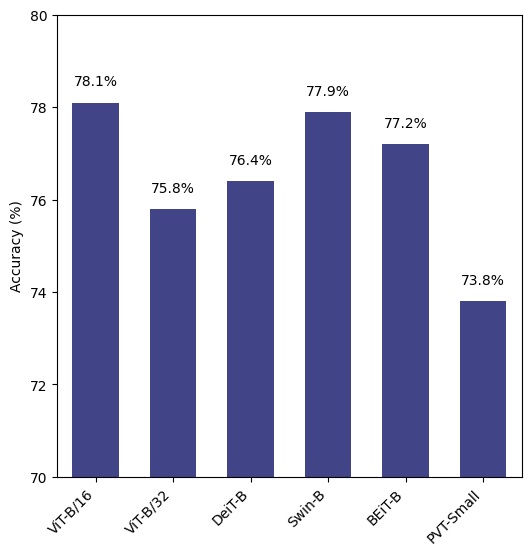
\includegraphics[width=0.6\linewidth]{Figures/pretrained_models.png}
    \caption{Classification Accuracy of Pre-Trained Models}
    \label{fig:pretrained_models}
\end{figure}

Overall, the results confirm that ViT-B/16 remains the most effective model for fine-tuned sleep stage classification, offering the highest accuracy and F1-score. However, models like DeiT-B and Swin-B provide viable alternatives with reasonable accuracy and improved computational efficiency. These findings highlight the trade-offs between model complexity, accuracy, and inference speed, which should be carefully considered in practical applications of automatic sleep stage classification. 

\section{Training and Tuning DCGAN for Synthetic Image Generation}

This section presents the findings on training and tuning DCGAN for synthetic image generation to address subject-to-subject variability and class imbalances in sleep stage classification. The DCGAN architectures listed in Table \ref{tab:dcgan_generator} and Table \ref{tab:discriminator} were trained to generate realistic PSG images, enhancing dataset diversity and improving model generalization. A visual comparison of original and synthetic images is shown in Figure \ref{fig:gan_generated}. The quality of the generated images was evaluated using Structural Similarity Index (SSIM), Fréchet Inception Distance (FID), and Mean Pairwise Euclidean Distance (MPED). The results provide insights into the effectiveness of DCGAN-based augmentation in generating synthetic sleep stage data.

\begin{figure}[H]
    \centering
    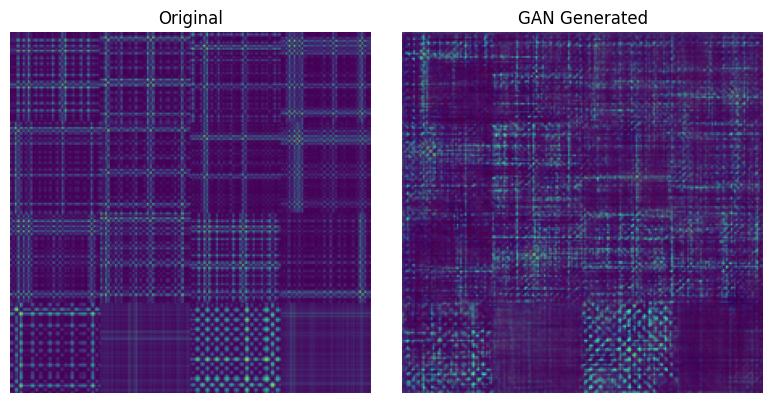
\includegraphics[width=0.6\linewidth]{Figures/gangenerated.png}
    \caption{Original Image vs. GAN Generated Synthetic Image }
    \label{fig:gan_generated}
\end{figure}

According to Figure \ref{fig:gan_generated}, the synthetic sleep stage images retained key structural patterns observed in real GASF transformed images, suggesting that the DCGAN successfully learned essential representations of different sleep stages. However, some variations were noted, such as minor artifacts and slight blurring in certain synthetic samples, which could impact their usefulness in model training. \\

\begin{table}[H]
    \centering
    \resizebox{\textwidth}{!}{ % Ensures the table fits within the page width
    \begin{tabular}{l l c c c c c}
        \toprule
        \textbf{Layer} & \textbf{Type} & \textbf{Kernel Size} & \textbf{Stride} & \textbf{Activation} & \textbf{Normalization} & \textbf{Output Shape} \\
        \midrule
        Input & Random Noise (100-dim) & - & - & - & - & (100,) \\
        Dense & Fully Connected \newline + Reshape & - & - & ReLU & BatchNorm & (14, 14, 1024) \\
        ConvTranspose1 & Transposed Conv2D & 4×4 & 2 & ReLU & BatchNorm & (28, 28, 512) \\
        ConvTranspose2 & Transposed Conv2D & 4×4 & 2 & ReLU & BatchNorm & (56, 56, 256) \\
        ConvTranspose3 & Transposed Conv2D & 4×4 & 2 & ReLU & BatchNorm & (112, 112, 128) \\
        ConvTranspose4 & Transposed Conv2D & 4×4 & 2 & ReLU & BatchNorm & (224, 224, 64) \\
        Output & Transposed Conv2D & 3×3 & 1 & Tanh & - & (224, 224, 3) \\
        \bottomrule
    \end{tabular}
    }
    \caption{DCGAN Generator Architecture}
    \label{tab:dcgan_generator}
\end{table}

\begin{table}[H]
    \centering
    \resizebox{\textwidth}{!}{ % Ensures the table fits within the page width
    \begin{tabular}{l l c c c c c}
        \toprule
        \textbf{Layer} & \textbf{Type} & \textbf{Kernel Size} & \textbf{Stride} & \textbf{Activation} & \textbf{Normalization} & \textbf{Output Shape} \\
        \midrule
        Input & PSG Image (224×224×3) & - & - & - & - & (224, 224, 3) \\
        Conv1 & Conv2D & 4×4 & 2 & LeakyReLU (0.2) & - & (112, 112, 64) \\
        Conv2 & Conv2D & 4×4 & 2 & LeakyReLU (0.2) & BatchNorm & (56, 56, 128) \\
        Conv3 & Conv2D & 4×4 & 2 & LeakyReLU (0.2) & BatchNorm & (28, 28, 256) \\
        Conv4 & Conv2D & 4×4 & 2 & LeakyReLU (0.2) & BatchNorm & (14, 14, 512) \\
        Conv5 & Conv2D & 4×4 & 2 & LeakyReLU (0.2) & BatchNorm & (7, 7, 1024) \\
        Flatten & Fully Connected & - & - & - & - & (1,) \\
        Output & Dense (Sigmoid) & - & - & Sigmoid & - & (1,) \\
        \bottomrule
    \end{tabular}
    }
    \caption{DCGAN Discriminator Architecture}
    \label{tab:discriminator}
\end{table}

We observe an SSIM score of 0.83, indicating high structural fidelity between real and synthetic images. The FID score of 18.7 suggests reasonable realism, though with room for improvement. Additionally, the MPED value of 5.62 confirms sufficient diversity, ensuring that synthetic samples enhance model generalization without redundancy.

\section{Effectiveness of GAN-Augmented Data}

This section presents the findings on the effectiveness of GAN-augmented data for sleep stage classification. The best-performing model, ViT-B/16, was fine-tuned on both the original dataset and a GAN-augmented dataset containing DCGAN-generated synthetic images. Performance comparisons assess whether synthetic data improves classification accuracy and generalization. Figure \ref{fig:synthetic_performance} summarizes the results, providing insights into the impact of GAN-based augmentation.

\begin{figure}[H]
    \centering
    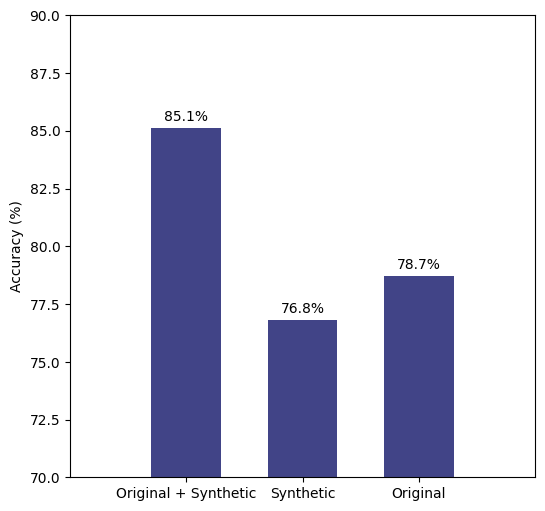
\includegraphics[width=0.6\linewidth]{Figures/synthetic_performance.png}
    \caption{Impact of GAN-Augmented Data on Sleep Stage Classification Performance}
    \label{fig:synthetic_performance}
\end{figure}

The results demonstrate that the combination of original and synthetic data significantly improves classification accuracy, with the mixed dataset yielding an accuracy of 85.1\%. This suggests that GAN-based data augmentation effectively enhances the model’s performance and generalization ability. Although the synthetic dataset alone achieved slightly lower accuracy (76.8\%) than the original dataset (78.7\%), its inclusion in the mixed dataset led to a notable improvement, highlighting the potential of synthetic data in addressing class imbalances and enhancing model robustness.

\section{Final Model}

Following Experiment 6, the ViT-B/16 model trained on the original + synthetic dataset using GASF and DWT at 128 Hz was identified as the best-performing model. To further evaluate its effectiveness, the model was tested on individual sleep stages. Figure \ref{fig:ds9} presents its performance across different sleep stages.

\begin{figure}[H]
    \centering
    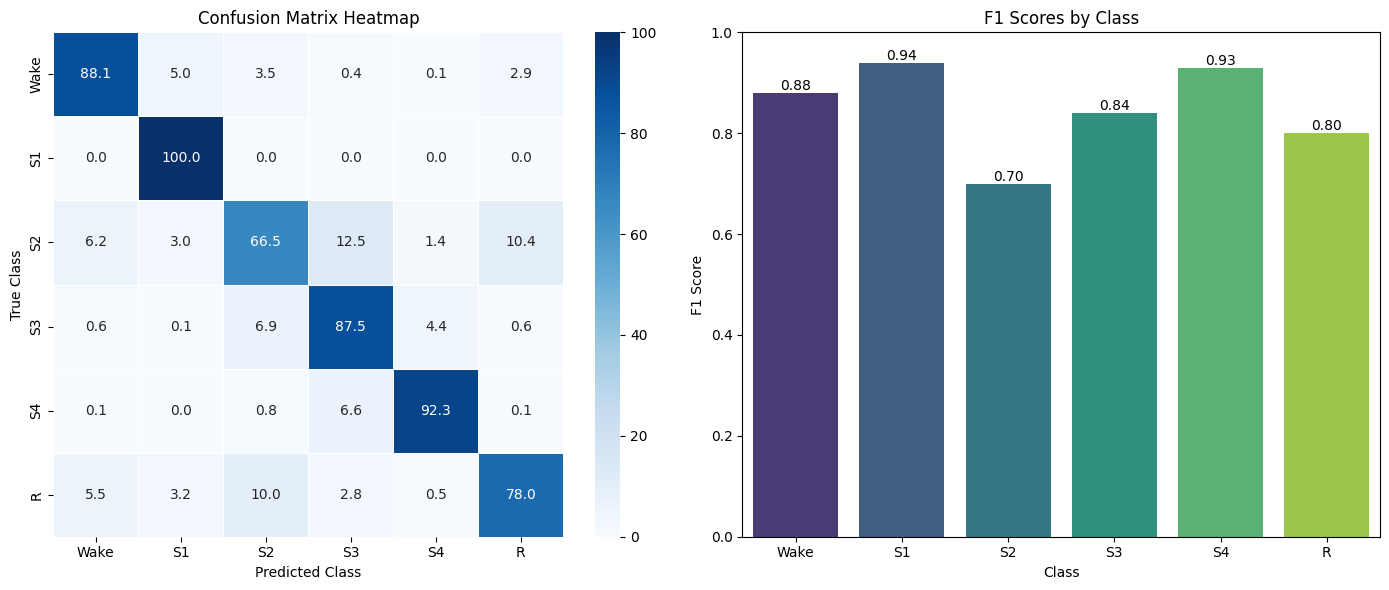
\includegraphics[width=1\linewidth]{Figures/ds9.png}
    \caption{Performance of the Final Model on Individual Sleep Stages}
    \label{fig:ds9}
\end{figure}

The final sleep stage classification model achieved an overall accuracy of 84.8\%, demonstrating its effectiveness in distinguishing between different sleep stages. The confusion matrix and F1 scores provide further insights into the model’s strengths and weaknesses across various classes. \\

The model performed exceptionally well in identifying S1 (light sleep), achieving an F1 score of 0.94, indicating a high balance between precision and recall. Similarly, S4 (deep sleep) was classified with a strong F1 score of 0.92, showing that the model effectively differentiates this stage from others. \\

Wake and REM (Rapid Eye Movement) sleep stages were also predicted with high reliability, obtaining F1 scores of 0.87 and 0.81, respectively. These results indicate the model’s robustness in distinguishing between wakefulness and different sleep states, which is crucial for sleep monitoring applications. \\

However, S3 (a transitional deep sleep stage) exhibited the lowest F1 score of 0.71, suggesting some confusion between S3 and adjacent sleep stages, particularly S2 and S4. The misclassification patterns indicate that the model sometimes confuses lighter and deeper sleep stages, which is a common challenge in sleep stage classification due to the gradual transition between these states. \\

To further assess the generalizability of the proposed sleep stage classification model, we evaluated its performance on the DS1-DS8 datasets. The results, summarized in Table \ref{tab:accuracy}, demonstrate the model's ability to maintain high classification accuracy across diverse datasets.

\begin{table}[H]
    \centering
    \begin{tabular}{|l|c|}
        \hline
        \textbf{DataSet} & \textbf{Accuracy} \\
        \hline
        Healthy (DS1) & 87.9\% \\
        Insomnia (DS2) & 92.8\% \\
        Bruxism (DS3) & 82.4\% \\
        Narcolepsy (DS4) & 88.2\% \\
        NFLE (DS5) & 86.6\% \\
        PLM (DS6) & 85.8\% \\
        RBD (DS7) & 81.0\% \\
        SDB (DS8) & 86.9\% \\
        All Subjects Combined (DS9) & 85.1\% \\
        \hline
    \end{tabular}
    \caption{Accuracy for Different Data Sets}
    \label{tab:accuracy}
\end{table}

The highest accuracy (92.8\%) was achieved on the Insomnia (DS2) dataset, suggesting that the model effectively distinguishes sleep stages in individuals with insomnia, potentially due to the clearer sleep stage transitions in this condition. The model also performed well on Narcolepsy (DS4) and Healthy (DS1) datasets, achieving 88.2\% and 87.9\% accuracy, respectively, demonstrating its effectiveness in both normal and disordered sleep patterns. \\

However, slightly lower accuracies were observed in datasets representing Bruxism (DS3, 82.4\%) and REM Behavior Disorder (RBD, DS7, 81.0\%), suggesting potential challenges in distinguishing sleep stages in subjects with these conditions. These variations could be attributed to irregular sleep patterns, movement artifacts, or differences in EEG characteristics associated with these disorders.\\

Despite these challenges, the model maintains strong generalization across all datasets, with accuracy ranging from 81.0\% to 92.8\%, reinforcing its applicability for diverse sleep conditions. 